\documentclass[11pt,a4paper]{article}

\usepackage[utf8]{inputenc}
\usepackage[T1]{fontenc}
\usepackage[margin=2.4cm]{geometry}
\usepackage{amsmath,amssymb}
\usepackage{graphicx,float}
\usepackage{caption}
\usepackage[dvipsnames,table]{xcolor}
\usepackage{booktabs}
\usepackage{tabularx}
\usepackage{array}
\usepackage{enumitem}
\usepackage{fancyhdr}
\usepackage{listings}
\usepackage{titlesec}
\usepackage[colorlinks=true,linkcolor=Indigo0G,urlcolor=Gold0G,citecolor=Indigo0G]{hyperref}
\usepackage{textcomp}

% Etiquetas en español (el paquete babel-spanish no está instalado en este entorno)
\renewcommand{\contentsname}{Índice}
\renewcommand{\figurename}{Figura}
\renewcommand{\tablename}{Tabla}
\renewcommand{\refname}{Referencias}
\renewcommand{\today}{23 de julio de 2026}

% ------------------------------------------------------------------
% Paleta corporativa 0G
% ------------------------------------------------------------------
\definecolor{Indigo0G}{HTML}{3B2E7E}
\definecolor{Purple0G}{HTML}{6A4C9C}
\definecolor{Gold0G}{HTML}{C9A227}
\definecolor{Light0G}{HTML}{F4F1FA}
\definecolor{Mid0G}{HTML}{D9D2EC}
\definecolor{Dark0G}{HTML}{1E1B2E}
\definecolor{Red0G}{HTML}{B23A48}
\definecolor{Green0G}{HTML}{2E7D5B}
\definecolor{Gray0G}{HTML}{8A8598}

% ------------------------------------------------------------------
% Encabezado / pie
% ------------------------------------------------------------------
\pagestyle{fancy}
\fancyhf{}
\lhead{\small\textcolor{Indigo0G}{\textbf{0G LockControl}} \textcolor{Gray0G}{— Diseño lógico y de firmware}}
\rhead{\small\textcolor{Gray0G}{\today}}
\cfoot{\small\textcolor{Gray0G}{\thepage}}
\renewcommand{\headrulewidth}{0.6pt}
\renewcommand{\headrule}{\hbox to\headwidth{\color{Mid0G}\leaders\hrule height \headrulewidth\hfill}}

% ------------------------------------------------------------------
% Títulos de sección con color
% ------------------------------------------------------------------
\titleformat{\section}{\Large\bfseries\color{Indigo0G}}{\thesection}{0.6em}{}
\titleformat{\subsection}{\large\bfseries\color{Purple0G}}{\thesubsection}{0.6em}{}
\titleformat{\subsubsection}{\normalsize\bfseries\color{Dark0G}}{\thesubsubsection}{0.6em}{}

% ------------------------------------------------------------------
% Estilo de código
% ------------------------------------------------------------------
\lstset{
  basicstyle=\ttfamily\footnotesize,
  breaklines=true,
  frame=single,
  rulecolor=\color{Mid0G},
  numbers=left,
  numberstyle=\tiny\color{Gray0G},
  keywordstyle=\color{Indigo0G}\bfseries,
  commentstyle=\color{Green0G}\itshape,
  stringstyle=\color{Gold0G},
  backgroundcolor=\color{Light0G},
  showstringspaces=false,
  captionpos=b,
  aboveskip=1em,
  belowskip=1em,
}

% Caja de nota
\newcommand{\nota}[1]{%
  \begin{center}\begin{minipage}{0.96\linewidth}
  \setlength{\fboxsep}{8pt}%
  \colorbox{Light0G}{\begin{minipage}{\dimexpr\linewidth-2\fboxsep}%
  \textcolor{Gold0G}{\textbf{Nota.}}~#1%
  \end{minipage}}%
  \end{minipage}\end{center}}

\newcommand{\dec}[1]{\textcolor{Green0G}{\textbf{#1}}}
\newcommand{\desc}[1]{\textcolor{Red0G}{\textbf{#1}}}

\captionsetup{labelfont={bf,color=Indigo0G},font=small}

% ==================================================================
\begin{document}

% ---------------- Portada ----------------
\begin{titlepage}
\centering
\vspace*{1.5cm}
{\color{Indigo0G}\rule{\linewidth}{2pt}}\\[0.4cm]
{\Huge\bfseries\color{Indigo0G} 0G LockControl}\\[0.3cm]
{\LARGE\color{Purple0G} Diseño lógico del firmware:\\[0.2em] entradas, estados, eventos y payload}\\[0.4cm]
{\color{Gold0G}\rule{\linewidth}{2pt}}\\[1.2cm]

{\large Alarma IoT dual — módulo \textbf{LSM110A} (STM32WL55 + Sigfox RC2)}\\[2cm]

\begin{tabular}{rl}
\textbf{\color{Indigo0G}Autor:} & José Francisco Díaz \\[0.3em]
\textbf{\color{Indigo0G}Área:} & I+D / Ingeniería — 0G IoT Solutions \\[0.3em]
\textbf{\color{Indigo0G}Proyecto:} & 0G-LockControl-LSM110A \\[0.3em]
\textbf{\color{Indigo0G}Documento:} & Especificación de máquina de estados y clasificación de eventos \\[0.3em]
\textbf{\color{Indigo0G}Versión:} & 0.1 (borrador de diseño) \\[0.3em]
\textbf{\color{Indigo0G}Fecha:} & \today \\
\end{tabular}

\vfill
{\small\color{Gray0G} Documento de diseño. Complementa a WP-01 «Codec del payload».
Cualquier cambio al contrato de bytes descrito aquí debe reflejarse en
\texttt{payload\_codec.\{h,c\}}, \texttt{payload\_parser.py} y los vectores de prueba.}
\end{titlepage}

\tableofcontents
\newpage

% ==================================================================
\section{Resumen ejecutivo}

Este documento le da estructura y coherencia a la lógica del firmware de
\textbf{0G LockControl}. Parte de tres entradas físicas (botón de armado, sensor
Hall de apertura y acelerómetro) y define de forma cerrada: las \textbf{variables
de estado}, los \textbf{eventos}, la \textbf{máquina de estados (FSM)}, la
\textbf{lógica de clasificación} del evento (resuelta con mapa de Karnaugh) y el
\textbf{mensaje de salida} con sus tres leyendas: \textsc{apertura},
\textsc{cierre} y \textsc{vandalismo}.

Las decisiones de diseño clave son:

\begin{itemize}[leftmargin=1.4em,itemsep=0.3em]
  \item \dec{Premisa de guardado:} el dispositivo sólo transmite si está
  \textbf{armado}. Si el usuario no presionó el botón al salir, la puerta puede
  abrirse y cerrarse sin generar ningún mensaje.
  \item \dec{Ventana de observación $T_{OBS}=10$~s:} tras la primera apertura se
  abre una ventana durante la cual se cuentan las aperturas ($N$) y se mide el
  desplazamiento máximo del acelerómetro ($\theta_{max}$). Al cierre de la
  ventana se clasifica y se transmite \emph{un solo} mensaje.
  \item \dec{Clasificación por 3 variables booleanas} $(C, M, P)$ que produce
  exactamente una de tres salidas mutuamente excluyentes (Sección~\ref{sec:kmap}).
  \item \dec{Medir «tiempo abierto» SÍ es viable} y se conserva, siempre que se
  implemente con el \textbf{RTC} (marca de tiempo en cada flanco) y \emph{no} con
  un timer de propósito general manteniendo el MCU despierto
  (Sección~\ref{sec:bateria}). El acercamiento ingenuo se \desc{descarta} y se
  justifica el porqué.
  \item \dec{La hora no viaja en el payload:} la aporta el backend Sigfox. El
  firmware sólo mide \emph{duración}.
\end{itemize}

% ==================================================================
\section{Entradas del sistema}

El dispositivo tiene tres fuentes de entrada, todas ya contempladas en el pinout
del LSM110A:

\begin{center}
\renewcommand{\arraystretch}{1.35}
\begin{tabularx}{\linewidth}{@{}l l l X@{}}
\toprule
\rowcolor{Indigo0G}
\textcolor{white}{\textbf{Entrada}} & \textcolor{white}{\textbf{Componente}} &
\textcolor{white}{\textbf{Pin / IRQ}} & \textcolor{white}{\textbf{Rol en la lógica}} \\
\midrule
Botón de inicio & Push-button & PA? / EXTI &
\textbf{Arma / desarma} el sistema. Al salir de casa, la persona lo presiona.
Es la llave maestra: sin armado, no hay mensajes. \\
\rowcolor{Light0G}
Apertura & Reed switch + DRV5032 (Hall) & PA1 / EXTI1 &
Detecta el \textbf{flanco de apertura/cierre} de la puerta. Fuente primaria del
evento y del conteo $N$. \\
Movimiento & LIS2DW12 (acelerómetro I\textsuperscript{2}C) & PA0 / EXTI0 (INT1) &
Mide el \textbf{desplazamiento angular} $\theta$ respecto a la posición de reposo
(\texttt{accel\_ref}). Discrimina apertura real de forcejeo. \\
\bottomrule
\end{tabularx}
\end{center}

\nota{El botón no aparece todavía en el pinout de la skill del proyecto; hay que
asignarle un GPIO con EXTI libre (p.\,ej.\ un PBx no usado) y su antirrebote.
El acelerómetro puede además usarse como fuente de \emph{wake} por umbral
(INT1), lo que permite que el MCU duerma en Stop2 hasta que algo se mueva.}

\subsection{Premisa de operación (la regla de oro)}

\begin{quote}
\itshape ``Sólo se transmite si el sistema está armado.''
\end{quote}

Esto se modela como una \textbf{guarda global}: cualquier flanco del sensor Hall
o del acelerómetro se ignora mientras \texttt{estado\_fsm == DESARMADO}. Es lo
que evita que el ir y venir normal de la casa (cuando hay gente adentro) inunde
el enlace Sigfox.

% ==================================================================
\section{Casos de uso}

La Figura~\ref{fig:casos} resume los actores y casos de uso. El \textbf{usuario}
arma y desarma; el \textbf{intruso} es un actor secundario que dispara las
detecciones; el \textbf{backend Sigfox} es el destino de todo mensaje. Todos los
casos de detección y el heartbeat culminan en «Enviar mensaje Sigfox»
(relación \texttt{«include»}).

\begin{figure}[H]
\centering
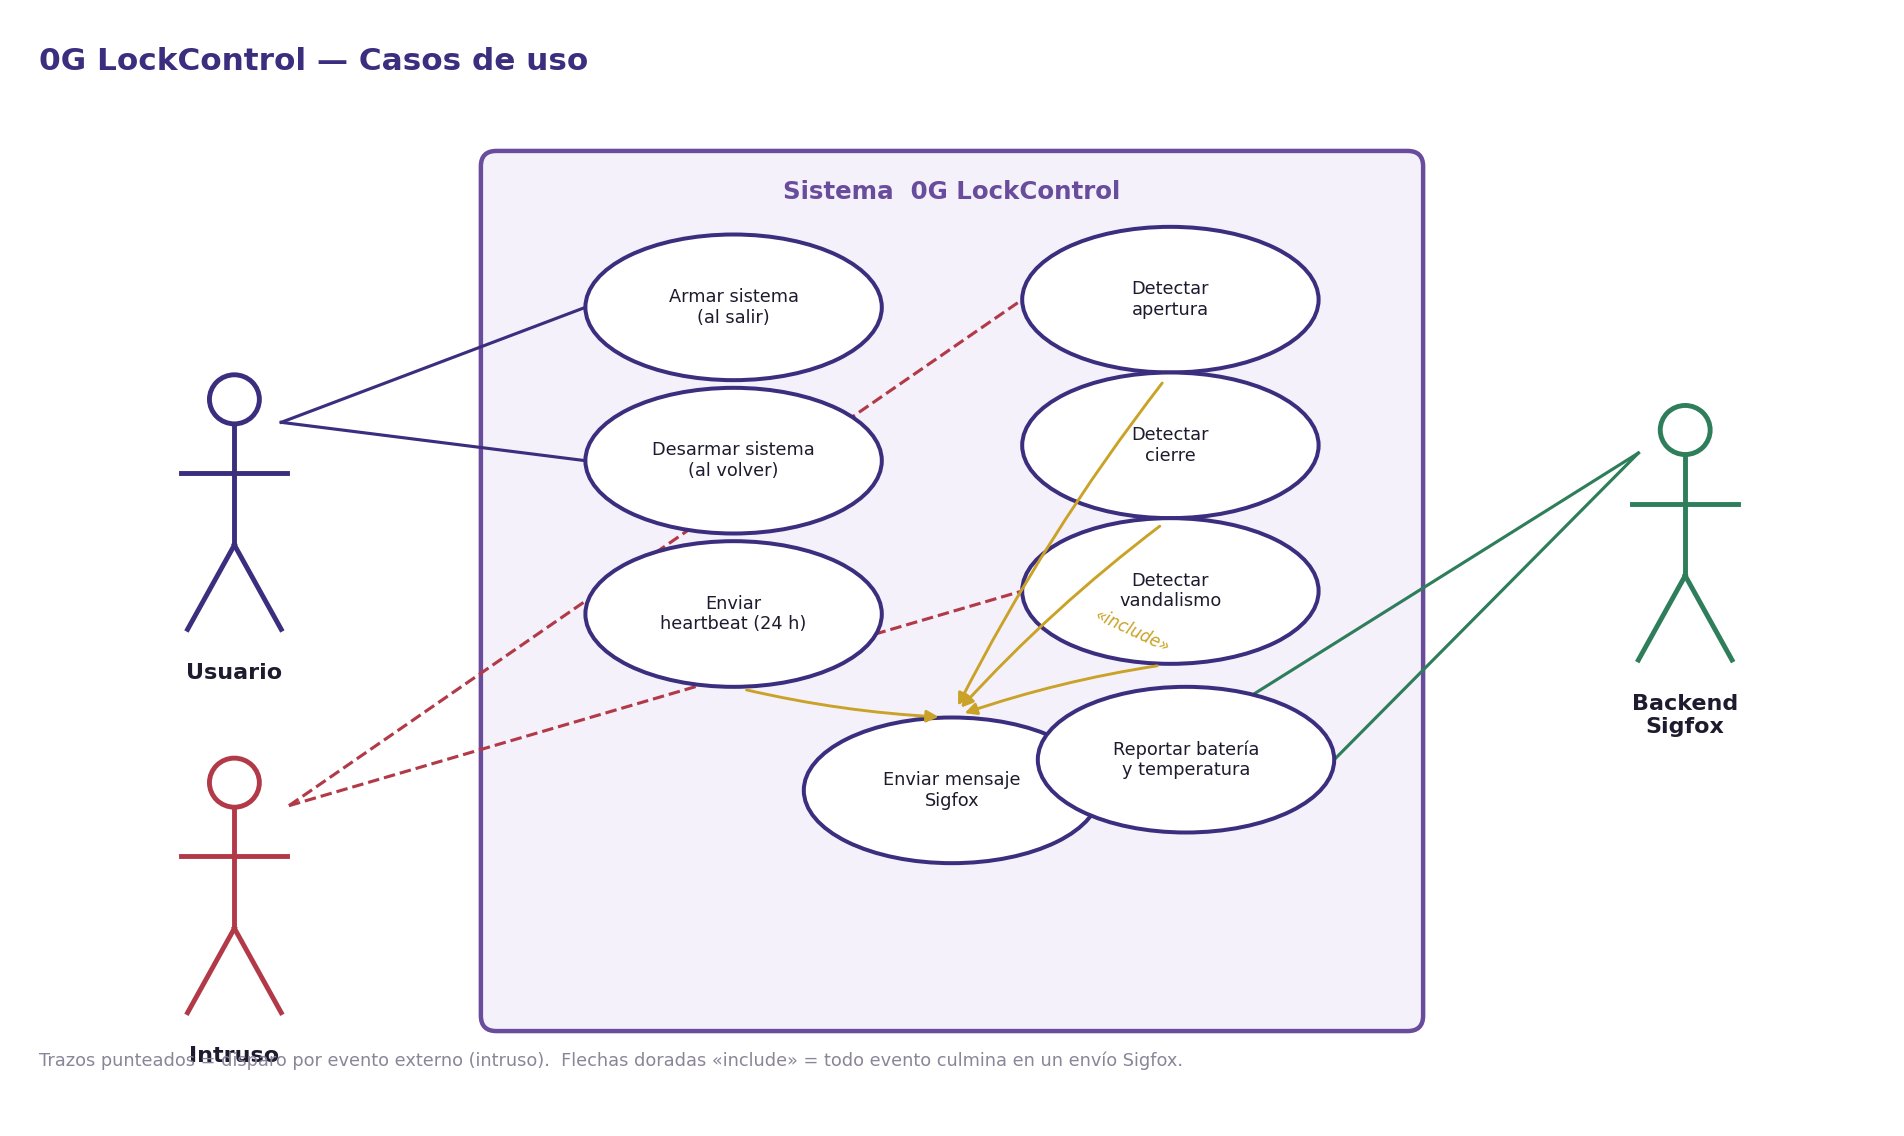
\includegraphics[width=0.95\linewidth]{figs/casos_uso.png}
\caption{Diagrama de casos de uso de 0G LockControl.}
\label{fig:casos}
\end{figure}

% ==================================================================
\section{Variables de estado temporales}
\label{sec:vars}

La lógica necesita mantener un pequeño conjunto de variables de estado durante la
ventana de observación:

\begin{center}
\renewcommand{\arraystretch}{1.3}
\begin{tabularx}{\linewidth}{@{}l l X@{}}
\toprule
\rowcolor{Indigo0G}
\textcolor{white}{\textbf{Variable}} & \textcolor{white}{\textbf{Símbolo}} &
\textcolor{white}{\textbf{Significado}} \\
\midrule
Estado de la puerta & $P$ & Abierta (1) / cerrada (0). Se actualiza en cada flanco Hall. \\
\rowcolor{Light0G}
Conteo de aperturas & $N$ & Número de flancos de apertura dentro de la ventana. \\
Desplazamiento máx. & $\theta_{max}$ & Máxima desviación del acelerómetro respecto a \texttt{accel\_ref} durante la ventana. \\
\rowcolor{Light0G}
Referencia de reposo & \texttt{accel\_ref} & Vector de gravedad capturado \textbf{al armar} (puerta cerrada). Es el ``cero'' contra el que se mide $\theta$. \\
Marca de apertura & $t_0$ & Valor del RTC en el flanco de apertura (para calcular el tiempo abierto). \\
\rowcolor{Light0G}
Tiempo abierto & $t_{ab}$ & Duración que la puerta permaneció abierta (sólo si hubo cierre). \\
\bottomrule
\end{tabularx}
\end{center}

De estas variables se derivan las tres \textbf{booleanas de decisión} que
alimentan la clasificación:

\begin{align}
C &= (N > N_{umbral}), \quad N_{umbral}=5 && \text{(``muchos ciclos'')}\\
M &= (\theta_{max} \geq \theta_{umbral}) && \text{(``movimiento significativo'')}\\
P &= \text{puerta abierta al cierre de la ventana} && \text{(estado final)}
\end{align}

% ==================================================================
\section{Eventos y tipos de mensaje}

\subsection{Eventos internos (disparadores de la FSM)}

\begin{center}
\renewcommand{\arraystretch}{1.25}
\begin{tabularx}{\linewidth}{@{}l X@{}}
\toprule
\rowcolor{Indigo0G}
\textcolor{white}{\textbf{Evento}} & \textcolor{white}{\textbf{Origen / efecto}} \\
\midrule
\texttt{EV\_BOTON}      & EXTI del botón — alterna armado/desarmado. \\
\rowcolor{Light0G}
\texttt{EV\_HALL}       & EXTI del Hall — flanco de apertura o cierre. \\
\texttt{EV\_ACCEL}      & INT1 del acelerómetro — movimiento por umbral. \\
\rowcolor{Light0G}
\texttt{EV\_T\_OBS}     & Fin de la ventana de observación (10~s) — dispara la clasificación. \\
\texttt{EV\_HEARTBEAT}  & Timer de 24~h — mensaje de vida. \\
\bottomrule
\end{tabularx}
\end{center}

\subsection{Tipos y subtipos de mensaje}

En el payload actual, el byte~0 (\texttt{tipo}) ya distingue \texttt{alarma}
(\texttt{0x01}) de \texttt{heartbeat} (\texttt{0x02}). Lo que \emph{falta} es
codificar la \textbf{leyenda} de la alarma. Se propone un byte de
\textbf{subtipo/evento} (Sección~\ref{sec:payload}):

\begin{center}
\renewcommand{\arraystretch}{1.25}
\begin{tabularx}{\linewidth}{@{}l l X@{}}
\toprule
\rowcolor{Indigo0G}
\textcolor{white}{\textbf{Mensaje}} & \textcolor{white}{\textbf{Código}} &
\textcolor{white}{\textbf{Cuándo}} \\
\midrule
\textsc{apertura}   & \texttt{evento=0x01} & La puerta quedó abierta al cierre de la ventana. \\
\rowcolor{Light0G}
\textsc{cierre}     & \texttt{evento=0x02} & La puerta se abrió y volvió a cerrarse dentro de la ventana. Lleva $t_{ab}$. \\
\textsc{vandalismo} & \texttt{evento=0x03} & Muchos flancos ($C$) pero sin apertura real ($\overline{M}$): forcejeo. \\
\rowcolor{Light0G}
heartbeat           & \texttt{tipo=0x02}   & Cada 24~h; sólo batería/temperatura. \\
\bottomrule
\end{tabularx}
\end{center}

% ==================================================================
\section{Máquina de estados (FSM)}

La Figura~\ref{fig:fsm} muestra la máquina completa. En reposo el dispositivo
vive en \texttt{ARMADO} dentro de \textbf{Stop2 ($\sim$3~$\mu$A)}, y sólo
despierta por un flanco Hall, por el acelerómetro o por el timer de heartbeat.

\begin{figure}[H]
\centering
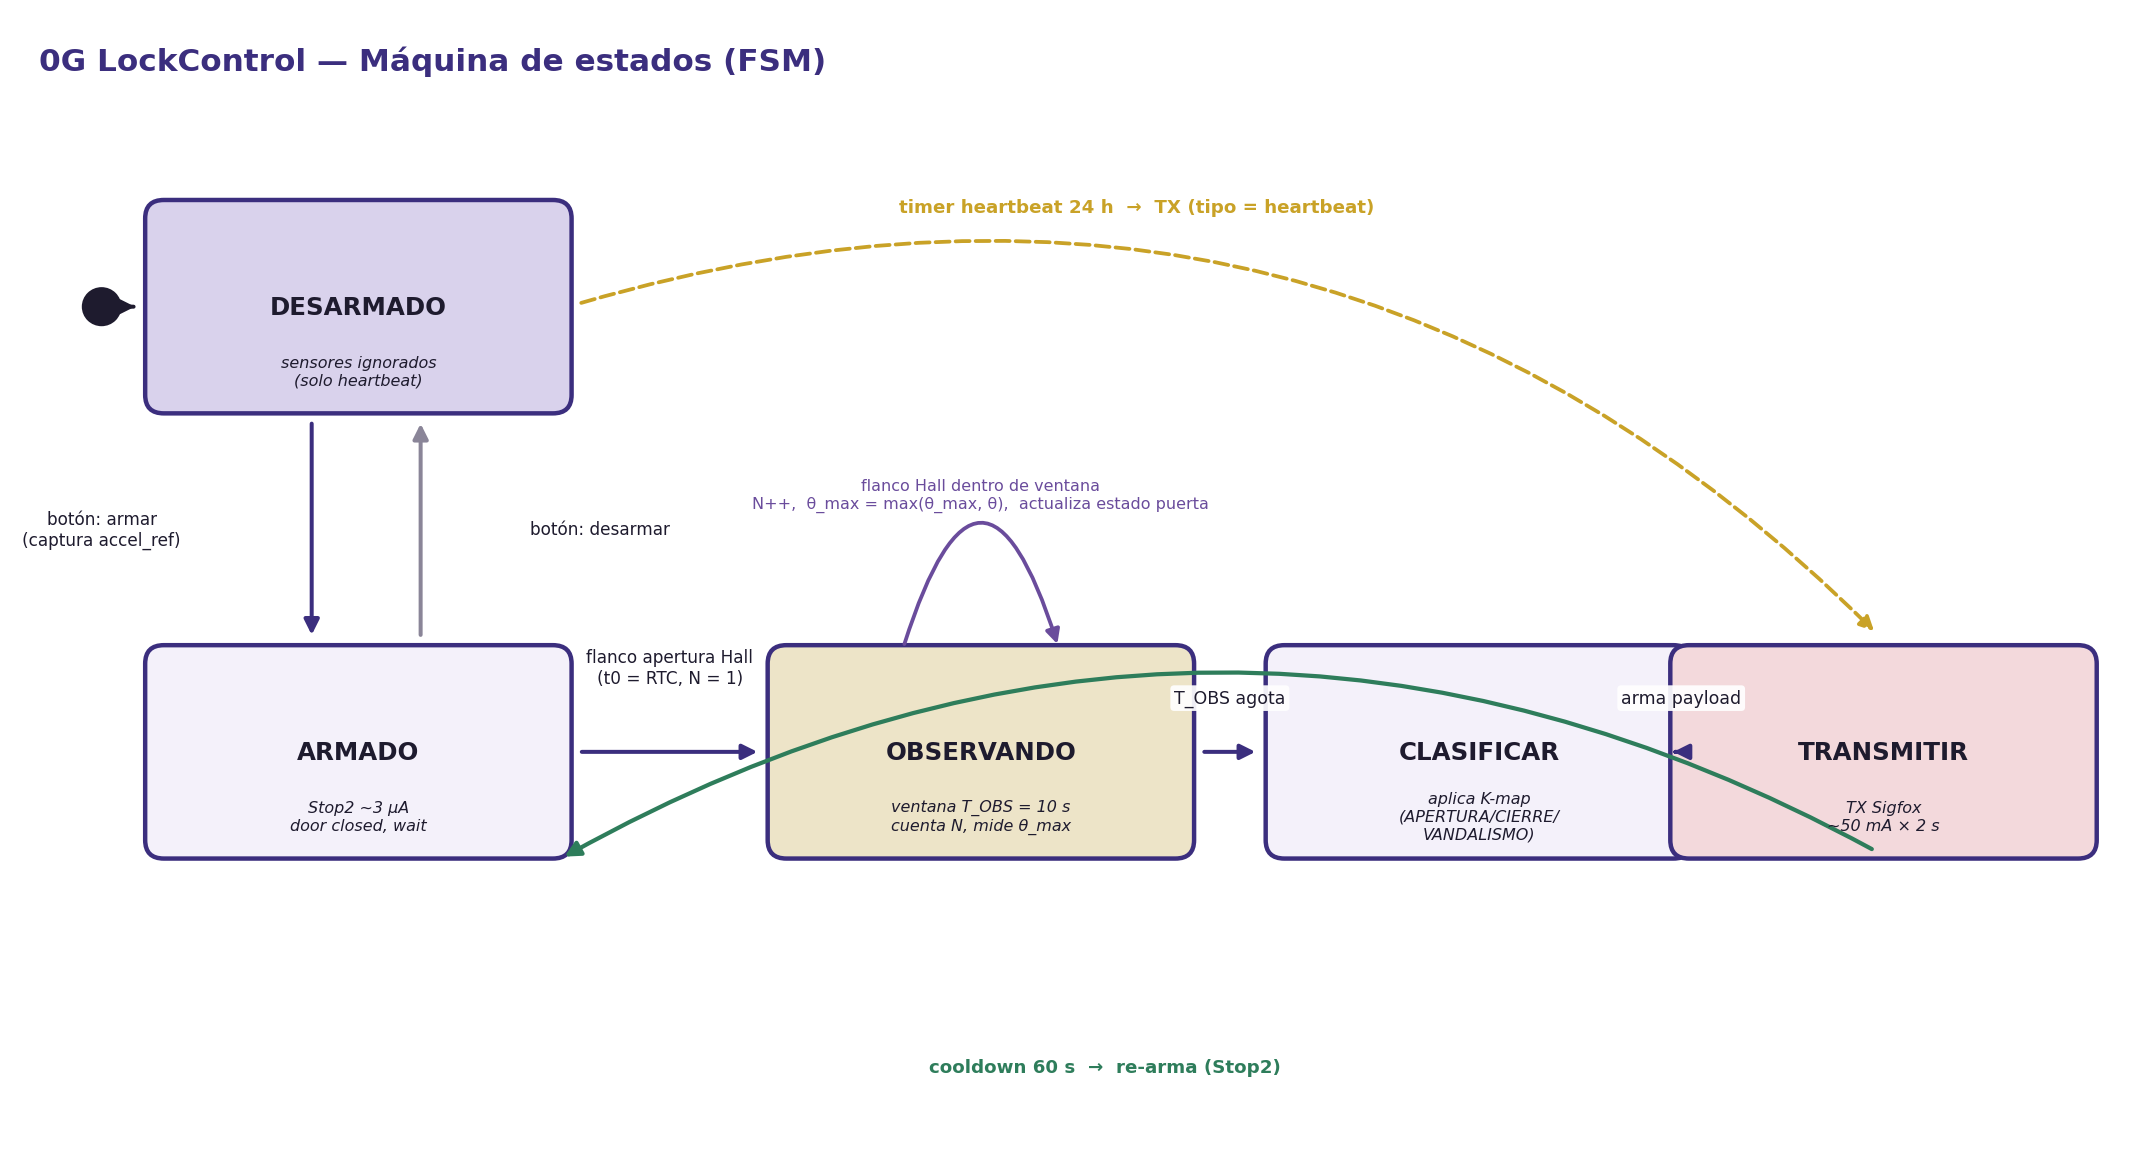
\includegraphics[width=\linewidth]{figs/estados_fsm.png}
\caption{Máquina de estados del firmware. La ventana de observación
($T_{OBS}$) sólo se arma tras una apertura estando \texttt{ARMADO}.}
\label{fig:fsm}
\end{figure}

\begin{description}[leftmargin=0em,style=nextline,itemsep=0.35em]
  \item[\texttt{DESARMADO}] Sensores ignorados (guarda de la premisa). Sólo corre
  el heartbeat. Se pasa a \texttt{ARMADO} con el botón, capturando
  \texttt{accel\_ref}.
  \item[\texttt{ARMADO}] Reposo de bajo consumo. Un flanco de apertura del Hall
  arranca la ventana ($t_0 = $ RTC, $N=1$) y pasa a \texttt{OBSERVANDO}.
  \item[\texttt{OBSERVANDO}] Durante $T_{OBS}=10$~s: cada flanco Hall incrementa
  $N$ y actualiza $P$; cada muestra del acelerómetro actualiza $\theta_{max}$.
  Al agotarse la ventana pasa a \texttt{CLASIFICAR}.
  \item[\texttt{CLASIFICAR}] Aplica la lógica de la Sección~\ref{sec:kmap} y arma
  el payload.
  \item[\texttt{TRANSMITIR}] TX Sigfox ($\sim$50~mA~$\times$~2~s). Aplica el
  \textbf{cooldown de 60~s} y re-arma (vuelve a \texttt{ARMADO}/Stop2).
\end{description}

% ==================================================================
\section{Lógica de clasificación: tabla de verdad y Karnaugh}
\label{sec:kmap}

La decisión de qué leyenda enviar depende de las tres booleanas $(C, M, P)$.
Con 3 variables hay $2^3=8$ combinaciones. La Tabla~\ref{tab:verdad} las lista
todas y la Figura~\ref{fig:kmap} muestra los mapas de Karnaugh.

\begin{table}[H]
\centering
\renewcommand{\arraystretch}{1.2}
\caption{Tabla de verdad de la clasificación. $C=(N>5)$, $M=(\theta_{max}\!\geq\!\theta_{umbral})$, $P=$ puerta abierta al final.}
\label{tab:verdad}
\begin{tabular}{ccc l l}
\toprule
\rowcolor{Indigo0G}
\textcolor{white}{$C$} & \textcolor{white}{$M$} & \textcolor{white}{$P$} &
\textcolor{white}{\textbf{Salida}} & \textcolor{white}{\textbf{Interpretación}} \\
\midrule
0 & 0 & 0 & \textsc{cierre}     & apertura suave, cerró (sin movimiento fuerte) \\
0 & 0 & 1 & \textsc{apertura}   & se abrió y quedó abierta \\
0 & 1 & 0 & \textsc{cierre}     & entrada/salida normal (abrió y cerró) \\
0 & 1 & 1 & \textsc{apertura}   & se abrió de verdad y quedó abierta \\
1 & 0 & 0 & \textsc{vandalismo} & muchos flancos, sin apertura real, cerrada \\
1 & 0 & 1 & \textsc{vandalismo} & muchos flancos, sin apertura real \\
1 & 1 & 0 & \textsc{cierre}     & muchos flancos pero abrió de verdad y cerró \\
1 & 1 & 1 & \textsc{apertura}   & muchos flancos y abrió de verdad, quedó abierta \\
\bottomrule
\end{tabular}
\end{table}

\begin{figure}[H]
\centering
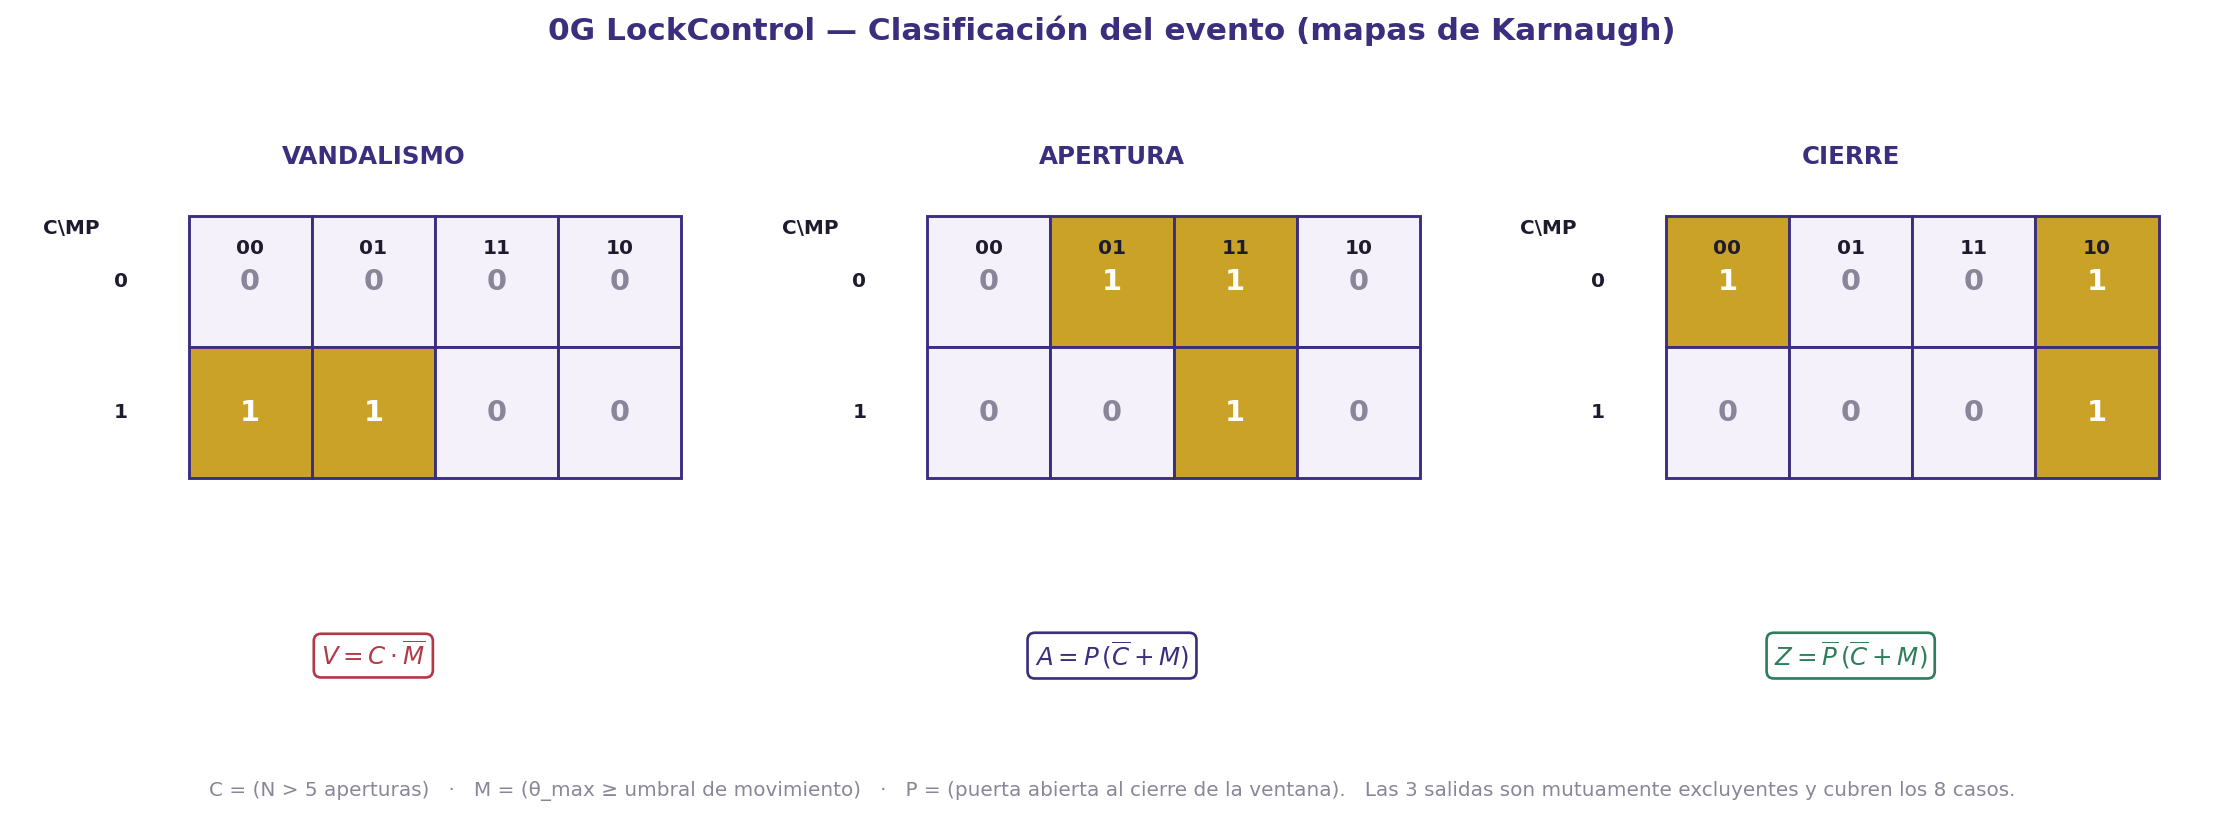
\includegraphics[width=\linewidth]{figs/karnaugh.png}
\caption{Mapas de Karnaugh de las tres salidas. Al simplificar se obtienen
expresiones muy compactas que se traducen directo a condicionales en C.}
\label{fig:kmap}
\end{figure}

Las ecuaciones minimizadas son:

\begin{align}
\textsc{vandalismo}:\quad V &= C \cdot \overline{M} \\
\textsc{apertura}:\quad A &= P \cdot (\overline{C} + M) \\
\textsc{cierre}:\quad Z &= \overline{P} \cdot (\overline{C} + M)
\end{align}

El criterio (la ``RCO'') es claro: \textbf{vandalismo} $=$ muchos flancos del
Hall \emph{sin} que el acelerómetro confirme que la puerta realmente se abrió.
Es decir, alguien forcejeó la puerta cerrada: el reed switch ``castañeteó''
varias veces pero la hoja no giró ($\theta_{max}$ bajo).

\nota{Con sólo 3 variables la minimización es casi trivial; el valor del
Karnaugh aquí es \emph{documental}: deja por escrito y verificable que las tres
salidas cubren los 8 casos y son mutuamente excluyentes, sin huecos ni
solapes.}

En C, la clasificación es literalmente:

\begin{lstlisting}[language=C,caption={Clasificación derivada del Karnaugh.}]
evento_t clasificar(uint16_t N, uint16_t th_max, bool puerta_abierta) {
    bool C = (N > N_UMBRAL);                 /* muchos ciclos          */
    bool M = (th_max >= THETA_UMBRAL);       /* movimiento real        */
    bool P = puerta_abierta;                 /* estado final           */

    if (C && !M)  return EV_VANDALISMO;      /* V = C . !M             */
    if (P)        return EV_APERTURA;        /* A = P . (!C + M)       */
    else          return EV_CIERRE;          /* Z = !P . (!C + M)      */
}
\end{lstlisting}

\subsection{¿Qué otros casos podría haber?}

Además de las tres leyendas y el heartbeat, quedan como \textbf{casos futuros}
(fuera del alcance inicial, pero fáciles de encajar en el mismo byte
\texttt{evento}):

\begin{itemize}[leftmargin=1.4em,itemsep=0.25em]
  \item \textbf{Batería baja} — cuando \texttt{bateria\_pct} cruza un umbral;
  puede piggy-back en el heartbeat en vez de gastar un mensaje propio.
  \item \textbf{Sabotaje del dispositivo (tamper)} — golpe/arranque de la pared
  detectado por el acelerómetro con la puerta \emph{cerrada}. Es distinto del
  vandalismo de puerta.
  \item \textbf{Puerta abierta prolongada} — recordatorio si $t_{ab}$ supera un
  límite; usar con cuidado por el presupuesto Sigfox.
\end{itemize}

% ==================================================================
\section{Análisis temporal: ventana de 10 s vs. 1 minuto}
\label{sec:tiempos}

Hay que separar \textbf{dos temporizadores distintos} que es fácil confundir:

\begin{center}
\renewcommand{\arraystretch}{1.3}
\begin{tabularx}{\linewidth}{@{}l l X@{}}
\toprule
\rowcolor{Indigo0G}
\textcolor{white}{\textbf{Temporizador}} & \textcolor{white}{\textbf{Valor}} &
\textcolor{white}{\textbf{Propósito}} \\
\midrule
Ventana de observación $T_{OBS}$ & \textbf{10 s} &
Agrega la ráfaga de flancos en \emph{un} evento, confirma que la apertura es real
y mide $N$ y $\theta_{max}$ antes de decidir. \\
\rowcolor{Light0G}
Cooldown de transmisión & \textbf{60 s} (ya decidido) &
Tiempo mínimo entre transmisiones. Es el \emph{anti-flood} que protege el
presupuesto Sigfox (130 msg/día). \\
\bottomrule
\end{tabularx}
\end{center}

\subsection{Por qué la ventana es de 10 s y no de 60 s}

La ventana cumple cuatro funciones: (1) \textbf{descartar glitches} (un flanco
aislado no es intrusión), (2) \textbf{agregar} una ráfaga en un solo mensaje,
(3) \textbf{capturar el forcejeo} (5 flancos en 10~s $=$ uno cada 2~s, cadencia
realista de alguien sacudiendo la puerta) y (4) \textbf{detectar el cierre}
dentro de la misma ventana para mandar \textsc{cierre} con $t_{ab}$.

\begin{itemize}[leftmargin=1.4em,itemsep=0.3em]
  \item \dec{A favor de 10 s:} \textbf{latencia baja}. En una alarma de
  seguridad quieres enterarte rápido; 10~s es un buen compromiso entre ``confirmar
  el evento'' y ``avisar pronto''. Además, como el \emph{anti-flood ya lo maneja
  el cooldown de 60~s} (decisión existente del proyecto) y el tope
  \texttt{daily\_msg\_limit=130}, \textbf{la ventana no necesita ser larga} para
  cuidar el presupuesto.
  \item \desc{En contra de 60 s:} retrasaría la alerta hasta un minuto y
  acoplaría ``observación'' con ``limitación de tasa'', que son cosas distintas.
  Sólo tendría sentido en una puerta muy ruidosa (muchas micro-aperturas
  legítimas) donde quieras promediar patrones más largos.
\end{itemize}

\dec{Recomendación:} $T_{OBS}=10$~s, \textbf{parametrizable} (\texttt{t\_obs\_ms}
en la config) por si en campo conviene ajustarlo. El ``análogo de 1 minuto'' que
mencionas equivale a fusionar la ventana con el cooldown; no se recomienda porque
degrada la latencia sin ganar nada (el presupuesto ya está protegido).

\begin{figure}[H]
\centering
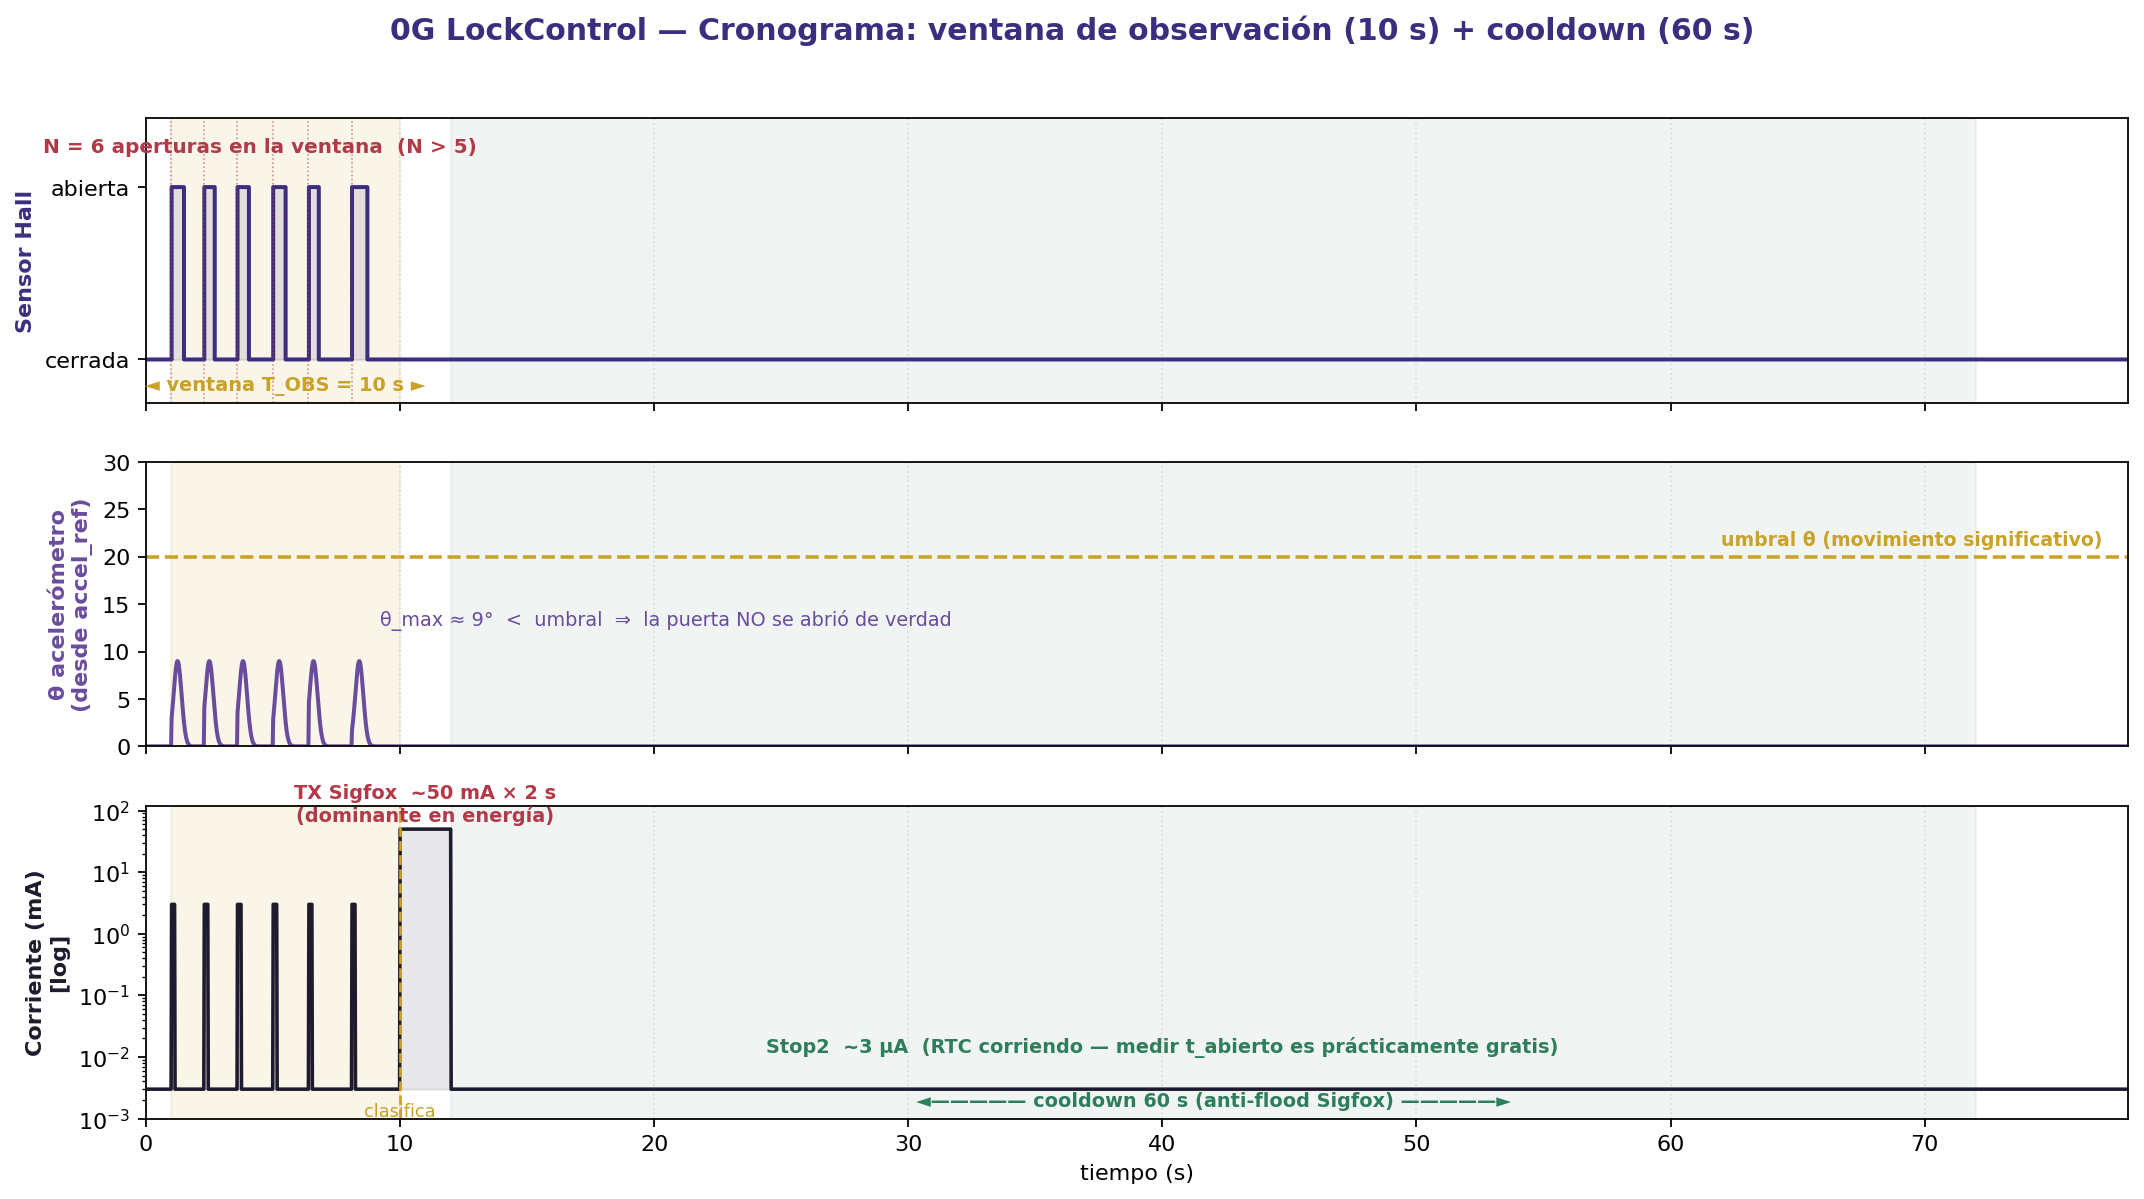
\includegraphics[width=\linewidth]{figs/cronograma.png}
\caption{Cronograma del escenario de vandalismo: 6 flancos del Hall en la
ventana de 10~s, $\theta$ por debajo del umbral (la puerta no se abrió de
verdad) $\Rightarrow$ \textsc{vandalismo}. Nótese que el pico de energía es la
transmisión Sigfox; el reposo en Stop2 es prácticamente plano.}
\label{fig:crono}
\end{figure}

% ==================================================================
\section{Medición del ``tiempo abierto'' y consumo}
\label{sec:bateria}

Preguntas dos cosas concretas: (a) ¿conviene guardar \emph{cuánto tiempo
permaneció abierta} la puerta? y (b) ¿arrancar un timer al abrir para esperar el
otro flanco descarga la batería?

\subsection{La respuesta corta}

\dec{Sí conviene medir $t_{ab}$, y sí es viable} — \textbf{siempre que se use el
RTC}, no un timer de propósito general con el MCU despierto. La diferencia de
consumo es de \textbf{tres órdenes de magnitud}.

\subsection{El porqué, con números}

El proyecto ya opera event-driven: \texttt{Stop2 ($\sim$3~$\mu$A) $\to$ wake por
INT $\to$ leer $\to$ TX ($\sim$50~mA~$\times$~2~s) $\to$ sleep}. La clave es
\emph{cómo} se mide la duración mientras la puerta está abierta:

\begin{itemize}[leftmargin=1.4em,itemsep=0.4em]
  \item \dec{Enfoque recomendado (RTC + Stop2):} al llegar el flanco de apertura
  se guarda \texttt{t0 = RTC}. El MCU \textbf{vuelve a dormir en Stop2}. Al
  llegar el flanco de cierre (EXTI lo despierta) se calcula
  $t_{ab} = \text{RTC} - t0$. Durante todo el intervalo el consumo es el de
  reposo ($\sim$3~$\mu$A), porque el RTC ya está corriendo. Medir cuesta
  \emph{dos lecturas de registro}: despreciable.
  \item \desc{Enfoque descartado (timer GP + MCU en Run):} mantener un timer de
  propósito general contando obliga al MCU a estar despierto (Run/Sleep con reloj
  rápido), del orden de \textbf{mA}, todo el tiempo que la puerta esté abierta.
\end{itemize}

\begin{table}[H]
\centering
\renewcommand{\arraystretch}{1.3}
\caption{Costo de energía de \emph{medir} el tiempo abierto, según el enfoque.
Batería CR2450 $\approx$ 600~mAh (verificar la parte). 1 TX $\approx$ 0.028~mAh.}
\label{tab:bateria}
\begin{tabular}{l r r r}
\toprule
\rowcolor{Indigo0G}
\textcolor{white}{\textbf{Puerta abierta}} &
\textcolor{white}{\textbf{RTC + Stop2 ($\sim$3\,$\mu$A)}} &
\textcolor{white}{\textbf{Timer GP + Run ($\sim$2\,mA)}} &
\textcolor{white}{\textbf{Factor}} \\
\midrule
1 minuto & $\sim$0.00005 mAh & $\sim$0.033 mAh ($\approx$1 TX) & $\sim$670$\times$ \\
\rowcolor{Light0G}
1 hora   & $\sim$0.003 mAh   & $\sim$2 mAh ($\approx$72 TX)    & $\sim$670$\times$ \\
8 horas  & $\sim$0.024 mAh   & $\sim$16 mAh ($\approx$576 TX)  & $\sim$670$\times$ \\
\bottomrule
\end{tabular}
\end{table}

\nota{La corriente en Run depende del reloj (aprox.\ $\sim$100~$\mu$A/MHz para el
Cortex-M4); a 16--48~MHz son $\sim$1.6--5~mA. El número exacto hay que sacarlo del
datasheet del STM32WL5x, pero lo robusto es el \emph{orden de magnitud}: mA
frente a $\mu$A. Si alguien deja la puerta abierta 8~h, el enfoque ingenuo se
come $\sim$16~mAh en \emph{un} evento; el enfoque con RTC, nada.}

\dec{Conclusión de diseño:} se conserva $t_{ab}$ en el payload (byte 11) y se
implementa con \textbf{captura de RTC en ambos flancos} + Stop2 en medio. El
acelerómetro, en modo bajo consumo, ronda unos pocos $\mu$A y puede muestrear
$\theta$ durante la ventana sin impacto relevante. \desc{Se descarta} el timer GP
con el MCU despierto.

% ==================================================================
\section{Secuencia de operación}

La Figura~\ref{fig:seq} traza el escenario de vandalismo de punta a punta: desde
que el usuario arma al salir, hasta la clasificación y el TX. Las flechas
punteadas rojas son eventos asíncronos (EXTI) que despiertan al MCU desde Stop2.

\begin{figure}[H]
\centering
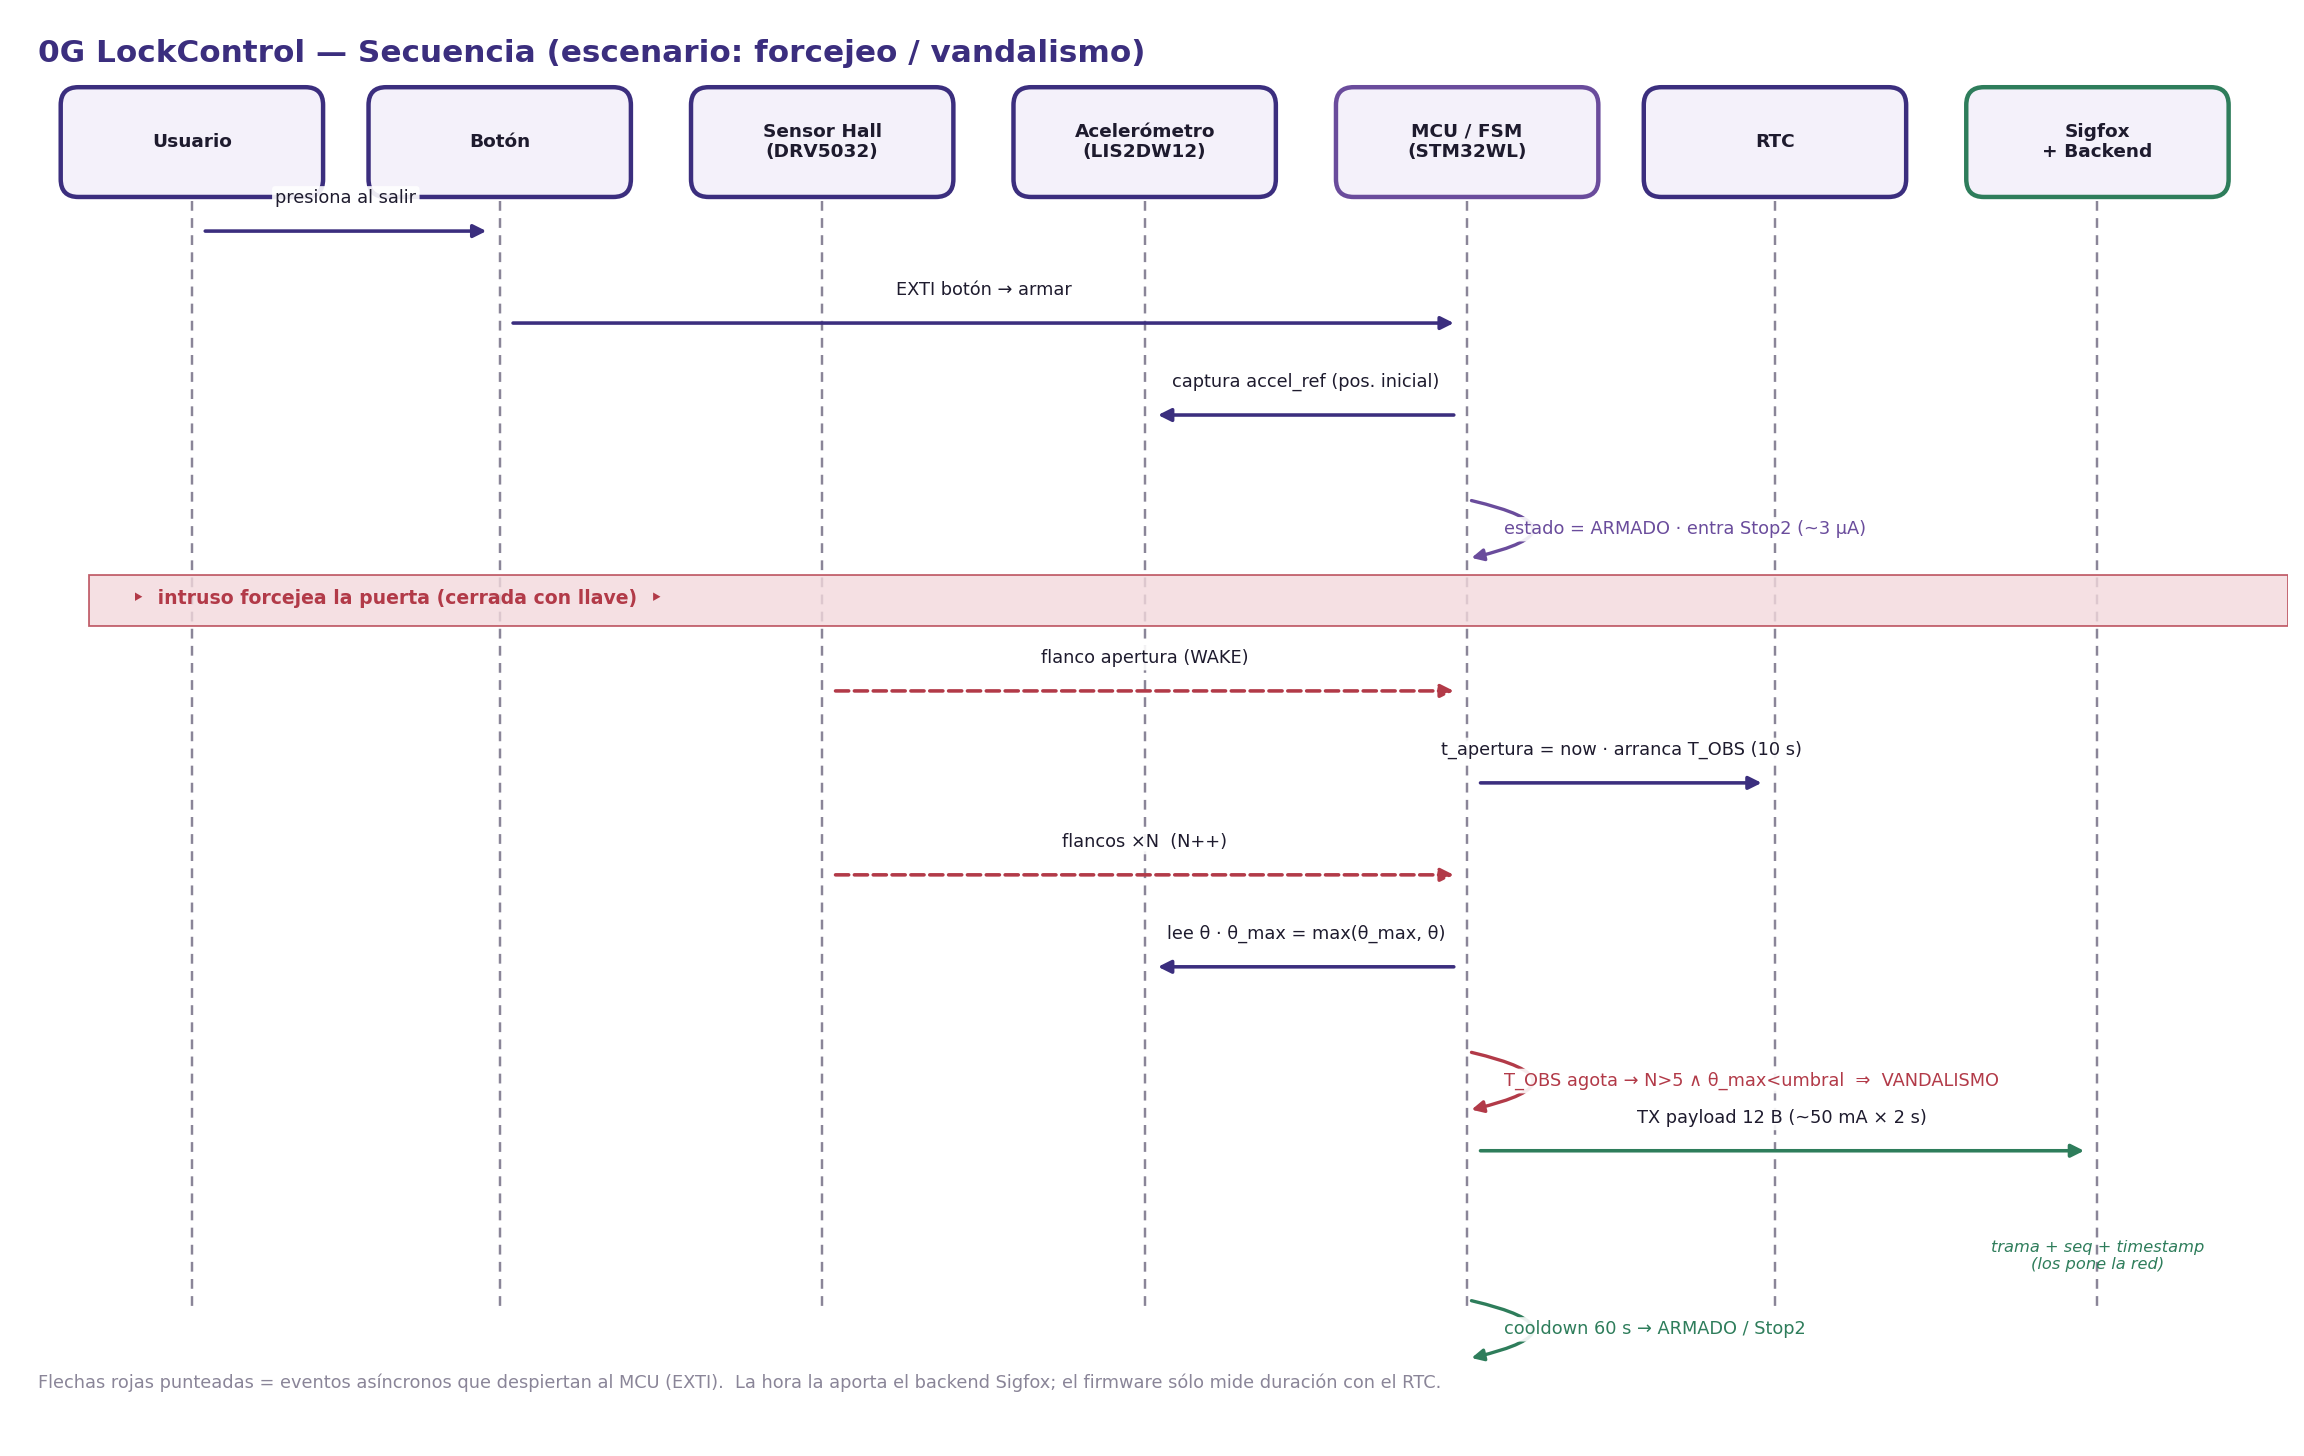
\includegraphics[width=\linewidth]{figs/secuencia.png}
\caption{Diagrama de secuencia (escenario: forcejeo / vandalismo).}
\label{fig:seq}
\end{figure}

% ==================================================================
\section{Propuesta de payload (extensión de WP-01)}
\label{sec:payload}

El payload actual (12 bytes) no tiene dónde poner la \textbf{leyenda} ni el
\textbf{tiempo abierto}. Se propone \textbf{reutilizar los dos bytes reservados}
(10--11) y \textbf{refinar} la semántica de dos campos, sin cambiar la longitud:

\begin{center}
\renewcommand{\arraystretch}{1.3}
\begin{tabularx}{\linewidth}{@{}c l l X@{}}
\toprule
\rowcolor{Indigo0G}
\textcolor{white}{\textbf{Byte}} & \textcolor{white}{\textbf{Campo}} &
\textcolor{white}{\textbf{Estado}} & \textcolor{white}{\textbf{Definición propuesta}} \\
\midrule
0     & \texttt{tipo}        & igual & \texttt{0x01} alarma / \texttt{0x02} heartbeat \\
\rowcolor{Light0G}
1     & \texttt{fuente}      & igual & bitfield accel/magnético (qué sensores participaron) \\
2--3  & \texttt{magnitud\_mg}& \textcolor{Purple0G}{\textbf{refinado}} & $\theta_{max}$: máx.\ desviación vs \texttt{accel\_ref} (mg) \\
\rowcolor{Light0G}
4     & \texttt{eje}         & igual & eje dominante del desplazamiento \\
5     & \texttt{magnetico}   & igual & $P$: 0 cerrado / 1 abierto (estado final) \\
\rowcolor{Light0G}
6     & \texttt{bateria\_pct}& igual & batería 0..100 \\
7     & \texttt{temp}        & igual & \texttt{temp\_c + 40} \\
\rowcolor{Light0G}
8--9  & \texttt{conteo}      & \textcolor{Purple0G}{\textbf{redefinido}} & $N$: aperturas en la ventana (BE) \\
10    & \texttt{evento}      & \textcolor{Green0G}{\textbf{NUEVO}} & \texttt{0x00} ninguno / \texttt{0x01} apertura / \texttt{0x02} cierre / \texttt{0x03} vandalismo \\
\rowcolor{Light0G}
11    & \texttt{t\_abierto\_s} & \textcolor{Green0G}{\textbf{NUEVO}} & duración abierta en s (0--255, saturado) \\
\bottomrule
\end{tabularx}
\end{center}

\begin{itemize}[leftmargin=1.4em,itemsep=0.25em]
  \item \textbf{Por qué liberar \texttt{conteo} para $N$:} Sigfox ya entrega un
  número de secuencia \emph{a nivel de red} (lo ve el backend), así que un
  contador monotónico en la app es redundante. Ese byte rinde más llevando el
  conteo de aperturas que pediste para el payload.
  \item \textbf{Compatibilidad:} en el heartbeat los bytes 10--11 quedan en
  \texttt{0x00}, igual que hoy, así que los vectores V4/V5 siguen válidos. Los
  vectores de alarma (V1--V3) habría que recalcularlos para incluir
  \texttt{evento}.
\end{itemize}

\nota{Este cambio toca el contrato de WP-01. Hay que actualizar
\texttt{payload\_codec.h/.c}, \texttt{payload\_parser.py} y \texttt{test\_vectors},
y volver a correr la validación C~$\leftrightarrow$~Python (5/5).}

% ==================================================================
\section{Variables de estado y control para el firmware}
\label{sec:firmware}

\subsection{Variables de estado (RAM, cambian en runtime)}

\begin{center}
\renewcommand{\arraystretch}{1.25}
\begin{tabularx}{\linewidth}{@{}l l X@{}}
\toprule
\rowcolor{Indigo0G}
\textcolor{white}{\textbf{Variable}} & \textcolor{white}{\textbf{Tipo}} & \textcolor{white}{\textbf{Descripción}} \\
\midrule
\texttt{estado\_fsm}   & \texttt{fsm\_state\_t} & Estado actual de la FSM. \\
\rowcolor{Light0G}
\texttt{armado}        & \texttt{bool}     & Sistema armado (guarda global). \\
\texttt{puerta\_abierta}& \texttt{bool}    & Estado actual del Hall ($P$). \\
\rowcolor{Light0G}
\texttt{n\_aperturas}  & \texttt{uint16\_t}& $N$: flancos de apertura en la ventana. \\
\texttt{theta\_max}    & \texttt{uint16\_t}& $\theta_{max}$ vs \texttt{accel\_ref} (mg). \\
\rowcolor{Light0G}
\texttt{accel\_ref[3]} & \texttt{int16\_t} & Vector de gravedad de reposo (al armar). \\
\texttt{t0\_rtc}       & \texttt{uint32\_t}& RTC en el flanco de apertura. \\
\rowcolor{Light0G}
\texttt{t\_abierto\_s} & \texttt{uint16\_t}& Duración abierta calculada (s). \\
\texttt{t\_ventana0}   & \texttt{uint32\_t}& Marca de inicio de la ventana $T_{OBS}$. \\
\rowcolor{Light0G}
\texttt{ultimo\_tx}    & \texttt{uint32\_t}& Timestamp del último TX (cooldown). \\
\texttt{msgs\_hoy}     & \texttt{uint8\_t} & Mensajes del día (presupuesto Sigfox). \\
\bottomrule
\end{tabularx}
\end{center}

\subsection{Banderas de evento (\texttt{volatile}, puestas por ISR/EXTI)}

\begin{center}
\renewcommand{\arraystretch}{1.2}
\begin{tabularx}{\linewidth}{@{}l X@{}}
\toprule
\rowcolor{Indigo0G}
\textcolor{white}{\textbf{Bandera}} & \textcolor{white}{\textbf{Fuente}} \\
\midrule
\texttt{flag\_boton}     & EXTI del botón. \\
\rowcolor{Light0G}
\texttt{flag\_hall}      & EXTI del Hall (+ dirección del flanco). \\
\texttt{flag\_accel}     & INT1 del LIS2DW12. \\
\rowcolor{Light0G}
\texttt{flag\_ventana}   & Fin de $T_{OBS}$ (alarma RTC / LPTIM). \\
\texttt{flag\_heartbeat} & Timer de 24~h. \\
\bottomrule
\end{tabularx}
\end{center}

\subsection{Parámetros de control (config en flash)}

Extienden la \texttt{device\_config\_t} que ya existe en el proyecto:

\begin{lstlisting}[language=C,caption={Config extendida y enums de la FSM.}]
typedef enum {
    ST_DESARMADO = 0,
    ST_ARMADO,
    ST_OBSERVANDO,
    ST_CLASIFICAR,
    ST_TRANSMITIR
} fsm_state_t;

typedef enum {
    EV_NINGUNO    = 0x00,
    EV_APERTURA   = 0x01,
    EV_CIERRE     = 0x02,
    EV_VANDALISMO = 0x03
} evento_t;

typedef struct {
    /* --- ya existentes --- */
    uint16_t accel_threshold_mg;  /* 200  -> tambien sirve como THETA_UMBRAL */
    uint16_t cooldown_seconds;    /* 60   -> anti-flood entre TX             */
    int8_t   tx_power_dbm;        /* 14                                      */
    uint8_t  heartbeat_hours;     /* 24                                      */
    uint8_t  daily_msg_limit;     /* 130                                     */
    /* --- NUEVOS para esta logica --- */
    uint16_t t_obs_ms;            /* 10000 -> ventana de observacion         */
    uint8_t  n_umbral;            /* 5     -> umbral de ciclos (vandalismo)  */
    uint8_t  debounce_ms;         /* 30-50 -> antirrebote del Hall/reed      */
} device_config_t;
\end{lstlisting}

\nota{El \textbf{antirrebote del Hall} (\texttt{debounce\_ms}) no es opcional: un
reed switch rebota, y sin filtrar, \emph{una} apertura real podría contarse como
varios flancos y disparar un ``vandalismo'' falso. Es la salvaguarda que hace
confiable la variable $N$.}

% ==================================================================
\section{Decisiones y descartes}

\begin{center}
\renewcommand{\arraystretch}{1.3}
\begin{tabularx}{\linewidth}{@{}l l X@{}}
\toprule
\rowcolor{Indigo0G}
\textcolor{white}{\textbf{Tema}} & \textcolor{white}{\textbf{Decisión}} & \textcolor{white}{\textbf{Razón}} \\
\midrule
Guarda de armado          & \dec{Sí}             & Evita inundar Sigfox con el tránsito normal. \\
\rowcolor{Light0G}
Ventana $T_{OBS}$         & \dec{10 s}           & Latencia baja + agrega ráfaga; el presupuesto ya lo cuida el cooldown. \\
Ventana de 1 min          & \desc{Descartada}    & Retrasa la alerta y acopla observación con rate-limit. \\
\rowcolor{Light0G}
Cooldown                  & \dec{60 s}           & Anti-flood (ya decidido en el proyecto). \\
Umbral de ciclos $N$      & \dec{5}              & Cadencia realista de forcejeo. \\
\rowcolor{Light0G}
Umbral $\theta$           & \dec{Reusar 200 mg}  & Discrimina apertura real; calibrar en campo. \\
Medir $t_{ab}$            & \dec{Sí, vía RTC}    & Costo despreciable ($\sim$3~$\mu$A). \\
\rowcolor{Light0G}
Timer GP + MCU en Run     & \desc{Descartado}    & Consumo en mA; descarga la batería (Tabla~\ref{tab:bateria}). \\
Hora en el payload        & \desc{Descartada}    & La aporta el backend Sigfox. \\
\rowcolor{Light0G}
Contador monotónico app   & \desc{Descartado}    & Sigfox ya da secuencia de red; se libera \texttt{conteo} para $N$. \\
\bottomrule
\end{tabularx}
\end{center}

% ==================================================================
\section{Conclusiones y siguientes pasos}

El sistema queda cerrado y coherente: tres entradas, una guarda de armado, una
ventana de 10~s que agrega y caracteriza el evento, y una clasificación de tres
salidas mutuamente excluyentes verificada con Karnaugh. La medición de tiempo
abierto se conserva porque, hecha con el RTC, no cuesta batería.

\textbf{Pendientes concretos:}
\begin{enumerate}[leftmargin=1.6em,itemsep=0.25em]
  \item Asignar el \textbf{GPIO del botón} (EXTI libre) en CubeMX y su antirrebote.
  \item \textbf{Calibrar} $\theta_{umbral}$ y \texttt{debounce\_ms} con la puerta real.
  \item Actualizar el \textbf{payload} (bytes 10--11 + semántica de 2--3 y 8--9) en
  \texttt{codec} y \texttt{parser}, y recalcular vectores V1--V3.
  \item Documentar esta lógica en el \textbf{Notion Hub} del proyecto y hacer
  commit al repo \texttt{0G-LockControl-\allowbreak LSM110A} (parando antes de \texttt{git push},
  como es la costumbre).
\end{enumerate}

\vfill
\begin{center}
{\color{Mid0G}\rule{0.5\linewidth}{1pt}}\\[0.3em]
{\small\color{Gray0G} 0G IoT Solutions — I+D · Documento de diseño 0G LockControl}
\end{center}

\end{document}
